\chapter{Projective Geometry} \label{chap:projgeo}

The treatment of projective geometry given throughout most of this chapter except
the last sections is taken from Audin's textbook \cite{audin}.

\section{Projective Spaces}

\begin{definition}
  Let $\vec{E}$ be a finite dimensional vector space. The \textit{projective space} $\Prj(\vec{E})$ deduced
  from $\vec{E}$ is the set of all $1$ dimensional linear subspaces of $\vec{E}$.
\end{definition}

\begin{remark}
  The dimension of $\Prj(\vec{E})$ is $\dim\vec{E}-1$. If $\vec{E}$ consists only of the point $0$, it does not
  contain any lines, and $\Prj(\vec{E})$ is empty. Thus it shall be implicitly assumed that $\dim\vec{E} \ge 1$.
  If $\dim\vec{E}=1$, $\vec{E}$ itself is a line, and thus the set of lines contains a unique element,
  $\Prj(\vec{E})$ is a point.
\end{remark}

\subsection{Projective Subspace}
A subset $V$ of $\Prj(\vec{E})$ is a projective subspace if it is an image of a non-zero vector subspace
$\vec{F}$ of $\vec{E}$.

\begin{prop}
  Let $V$ and $W$ be two projective subspaces of $\Prj(\vec{E})$.
  
  \begin{itemize}
    \item If dim $V$ + dim $W$ $\ge$ dim $\Prj(\vec{E})$, then $V\cap W$ is not empty.
    \item Let $H$ be a hyperplane of $\Prj(\vec{E})$, and let $m$ be a point not in $H$. Every
      line through $m$ intersects $H$ at a unique point.
  \end{itemize}

\end{prop}

\begin{proof}
  Let $\vec{F}$ and $\vec{G}$ be the vector subspaces of $\vec{E}$ from which $V$ and $W$ were deduced, i.e.
  $V=\Prj(\vec{F})$, and $W=\Prj(\vec{G})$. The statement can be translated into vector subspaces as
  \begin{align*}
    & (\text{dim }\vec{F}-1)+(\text{dim }\vec{G}-1)\ge(\text{dim }\vec{E}-1)\\
    \implies& \text{dim }\vec{F}+\text{dim }\vec{G}\ge\text{dim }\vec{E}+1
  \end{align*}
  We can use the linear algebraic properties to further deduce that:
  \[
    \dim\vec{F}+\dim\vec{G}=\dim(\vec{F}+\vec{G})+\dim(\vec{F}\cap \vec{G})
    \le\dim\vec{E}+\dim(\vec{F}\cap \vec{G})
  \]
  Therefore,
  \[
    \text{dim }(\vec{F}\cap \vec{G})\ge1
  \]
  This can be translated back into projective geometry to conclude that $V\cap W$ is not empty.

  Now, to prove the second property, let $\vec{J}$ be the vector hyperplane of which $H$ is image of.
  The point $m$ is the image of a line $\ell$ in $\vec{E}$, not contained in the hyperplane $\vec{J}$.
  The assertion, translated in terms of linear algebra, is that any plane $\vec{P}$ containing $\ell$
  meets $\vec{J}$ along a unique line. Since $\ell$ is not in $\vec{J}$, we have $\vec{P}+\vec{J}=\vec{E}$. Hence,
  \begin{align*}
    \dim(\vec{P}\cap\vec{J}) &= \dim\vec{P}+\dim\vec{J}-\dim(\vec{P}+\vec{J})\\
                             &= 2+\dim\vec{E}-1-\dim\vec{E}=1
  \end{align*}
\end{proof}

\subsection{Projective Transformation}

\begin{definition}
  Let $\vec{E}$ and $\vec{E}'$ be two vector subspaces, and ${p\colon\vec{E}\setminus\{0\}\to\Prj(\vec{E})}$ and
  ${p'\colon\vec{E}'\setminus\{0\}\to\Prj(\vec{E}')}$ be the two projections. A \textit{projective transformation}
  ${g\colon\Prj(\vec{E})\to\Prj(\vec{E}')}$ is a mapping such that there exists a linear isomorphism
  ${f\colon\vec{E}\to\vec{E}'}$ with $p'\circ f=g\circ p$.
\end{definition}

\begin{prop}
  The set of projective transformations from $\Prj(\vec{E})$ to itself, $\PGL(\vec{E})$, is a group under
  composition.
\end{prop}

\begin{proof}
  From the definitions, the projective transformation that descends from identity map of $\vec{E}$
  forms the identity of the group. For any projective tranformation $g$ that descends from a
  linear isomorphism $f$, the transformation $g'$ that descends from $f^{-1}$ will act as its
  inverse. Since functional composition obeys associativity, $\PGL(\vec{E})$ is a group under
  composition.
\end{proof}

\subsection{Homogeneous Coordinates and Projective Frames}

Given a basis of vector space $\vec{E}$, the vectors in $\vec{E}$ can be descirbed by their coordinates with
respect to the basis. 

\begin{definition}
  A point $m$ in $\Prj(\vec{E})$ can be described by the non-zero vector that generates the line $m$. In a
  n-dimensional projective space $\Prj(\vec{E})$, the $(n+1)$ tuples $[x_1:\dots:x_{n+1}]$ and
  $[x'_1:\dots:x'_{n+1}]$ represent the same point iff there exists a non-zero scalar $\lambda$
  such that $x_i=\lambda x'_i$ for all $i$.
\end{definition}

In a projective space $\Prj(\vec{E})$ with dimension $n$, we actually need $n+2$ points to uniquely determine
the basis of the underlying space $\vec{E}$, which will be proved in the next lemma. It will also
justify the next definition.

\begin{definition}
  If $\vec{E}$ is a vector space of dimension $n+1$, a \textit{projective frame} of $\Prj(\vec{E})$ is a set of
  $n+2$ points  $(m_0,\dots,m_{n+1})$ such that $m_1,\dots,m_{n+1}$ are the images of the
  vectors $\vec{e}_1,\dots,\vec{e}_{n+1}$ in a basis of $\vec{E}$, and $m_0$ is the image of
  $\vec{e}_1+\dots+\vec{e}_{n+1}$.
\end{definition}

\begin{lemma}
  Let $(m_0,\dots,m_{n+1})$ be a projective frame of $\Prj(\vec{E})$. If the two bases of $\vec{E}$
  $(\vec{e}_1,\dots,\vec{e}_{n+1})$ and $(\vec{e'}_1,\dots,\vec{e'}_{n+1})$ are such that $p(\vec{e}_i)=p(\vec{e'}_i)=m_i$ and
  $p(\vec{e}_1+\dots+\vec{e}_{n+1})=p(\vec{e'}_1+\dots+\vec{e'}_{n+1})=m_0$, then they are proportional.
\end{lemma}

\begin{proof}
  Consider the points $m_i$ of $\Prj(\vec{E})$. Since the vectors $\vec{e}_i$ and $\vec{e'}_i$ both generate the line
  $m_i$, $\vec{e}_i=\lambda_i \vec{e'}_i$ for some non-zero $\lambda_i$. Using the $(n+2)$-th point, we can
  conclude that 
  \[
    (\vec{e}_1+\dots+\vec{e}_{n+1})=\lambda(\vec{e'}_1+\dots+\vec{e'}_{n+1})
  \]
  Thus,
  \[
      \lambda_1\vec{e}_1+\dots+\lambda_{n+1}\vec{e}_{n+1}=\lambda(\vec{e}_1+\dots+\vec{e}_{n+1})
  \]
  As we are dealing with a basis, $\lambda_i=\lambda$. Thus two bases are proportional.
\end{proof}

\begin{prop}
  Let $\Prj(\vec{E})$ and $\Prj(\vec{E}')$ be two projective spaces of dimension $n$. Any projectivve mapping from
  $\Prj(\vec{E})$ to $\Prj(\vec{E}')$ maps a projective frame of $\Prj(\vec{E})$ onto a projective frame of $\Prj(\vec{E}')$.
\end{prop}

\section{Fundamental Theorem of Projective Geometry}

\begin{theorem}[Fundamental Theorem of Projective Geometry] \label{thm:fundprojgeo}
    Let $(a_1,\dots,a_{n+1})$ and $(b_1,\dots,b_{n+1})$ be two sets of points in $\Prj(\R^n)$ such
  that none of the $a_i$ and $b_i$ belong to the projective subspace defined by $n-1$ of the others
  in their respective sets. Then there exists a unique projective transformation
  $f\colon\Prj(\R^n)\to\Prj(\R^n)$ such that, $f(a_i)=b_i$ for all $i=1,\dots,n+1$.
\end{theorem}

\begin{proof}
  The set of points $(a_i)$ and $(b_i)$ are both projective frames of $\Prj(\R^n)$. Let
  $(\vec{e}_1,\dots,\vec{e}_n)$, $(\vec{e'}_1,\ldots,\vec{e'}_n)\in\R^n$ be the basis that generate the frames
  $(a_i)$ and $(b_i)$ respectively. We know that there exists a unique isomorphism
  $f\colon\R^n\to\R^n$ such that $f(\vec{e}_i)=\vec{e'}_i$. The projective transformation $g$
  that descends from $f$ will map the first frame to the second.

  To prove the uniqueness: let $f$ and $f'$ two such projcetive transformations. The projective
  transormation $g^{-1}\circ g'$ from $\Prj(\R^n)$ into itself keeps the frame invariant. Thus
  it is the identity transformation.
\end{proof}

\begin{theorem}[Desargues's Theorem]
  Let $\triangle ABC$ and $\triangle A'B'C'$ be triangles in $\R^2$ such that the lines $AA'$,
  $BB'$, and $CC'$ meet at point $U$. Let $BC$ and $B'C'$ meet at $P$, $CA$ and $C'A'$ at $Q$,
  and $AB$ and $A'B'$ at $R$. Then $P$, $Q$, and $R$ are collinear.
\end{theorem}

\begin{figure}[H]
  \center
  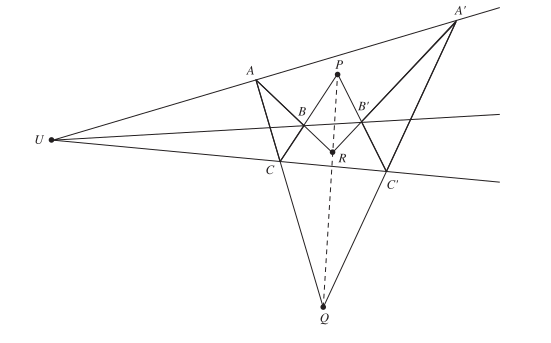
\includegraphics[width=0.75\linewidth]{pictures/desargues.png}
  \caption{Figure from \cite{brannan}.}
\end{figure}

\begin{proof}
  We will prove the theorem for the special case where $A=[1:0:0]$, $B=[0:1:0]$, $C=[0:0:1]$,
  and $U=[1:1:1]$. From the fundamental theorem of projective geometry, we know that it will be
  congruent to any other configuration. We can use the fact that projective congruence preserves
  projrctive properties, to deduce that the theorem holds in general.

  The line $AU$ has the equation $y=z$. Since $A'$ lies on $AU$, it must have coordinates
  $[a:b:b]$, where $b\ne 0$, since $A'\ne A$. We can also wirte $A'=[p:1:1]$, where $p=a/b$.
  Similary, $B'=[1:q:1]$, and $C'=[1:1:r]$.

  Now to find the point $P$, we find the equation of the line $BC$.
  \[
    \begin{vmatrix}
      x & y & z\\
      1 & q & 1\\
      1 & 1 & r
    \end{vmatrix}
    =0\implies (qr-1)x-(r-1)y+(1-q)=0
  \]
  Substituting $x=0$ in the equation for the line $B'C'$, we get $(r-1)y=(1-q)z$, which immplies
  $P=[0:1-q:r-1]$. Similarly we find that $Q=[1-p:0:r-1]$, and $R=[1-p:q-1:0]$.

  To check the collinearity of $P$, $Q$, and $R$:
  \begin{align*}
    \begin{vmatrix}
      0   & 1-q & r-1 \\
      1-p & 0   & r-1\\
      1-p & q-1 & 0
    \end{vmatrix}
    = -(1-q)(1-p)(1-r)+(r-1)(1-p)(q-1) = 0
  \end{align*}

  i.e $P$, $Q$, and $R$ are collinear.
\end{proof}

\begin{prop}
  There is a unique projective conic through any given set of five points, no three of which are
  collinear.
\end{prop}

\begin{proof}
 By the fundamental theorem of projective geometry, there exists a projective transformation
 $t$ which maps the four out of given five points to the points $[1:0:0]$, $[0:1:0]$, $[0:0:1]$
 and $[1:1:1]$. Let $[a:b:c]$ be the image of the fifth point under $t$. Since projective
 transformations preserve collinearity, no three of the five points are collinear, and also
 it can be deduced that $a$, $b$ and $c$ are non-zero, since if it were so, it would be collinear
 with other two points.

 \vspace{1ex}

 \noindent
 Let the conic that passes through these 5 points be of the form
 \[
   Ax^2+Bxy+Cy^2+Fxz+Gyz+Hz^2
 \]
 By substituting the points $[1:0:0]$, $[0:1:0]$, and $[0:0:1]$, the equation can be reduced
 to the form
 \[
   Bxy+Fxz+Gyz=0
 \]
 Since the porjective concic also passes through $[1:1:1]$ and $[a:b:c]$, we get the equations
 \[
   B+F+G=0
 \]
 and
 \[
   Bab+Fac+Gbc=0
 \]
 Solving these simultaneous equations, we get
 \[
   F=-G\frac{ab-bc}{ab-ac}
 \]
 and
 \[
   B= -G\frac{ac-bc}{ac-ab}
 \]
 It follows that the conic is of the form
 \[
   -G\frac{ac-bc}{ac-ab}xy-G\frac{ab-bc}{ab-ac}xz+Gyz=0
 \]
 or
 \[
   c(a-b)xy+b(c-a)xz+a(b-c)yz=0
 \]
 Since the conic is uniquely determined by the fifth point, it follows that it is unique.\\
\end{proof}

\begin{remark}
  \textbf{The Standard Projective Conic}

  The projective conic $E=\{[x:y:z]:xy+yz+zx=0\}$ is called the standard projective conic.
  It passes through the traingle of reference formed by the points $[1:0:0]$, $[0:1:0]$, and
  $[0:0:1]$. This fact can be used to simplify calculations involving projcetive conics.

  All the points on the conic except than $[1:0:0]$ can be parameterized as $[t^2+t:t+1:-t]$,
  where $t\in\R$. All points on $\vec{E}$ satisfy $xy+yz+zx=0$. Suppose $y\ne 0$, let $t=x/y$. Then
  $x=ty$, and so
  \begin{align*}
    & (ty)y+yz+z(ty)=0 \\
    \implies & ty+(t+1)z=0 \\
    \implies & y=-\frac{t+1}{t}z, x=-(t+1)z
  \end{align*}

  Thus the point has homogeneous coordinates $\left[-(t+1)z:-\frac{t+1}{t}z:z\right]$, which can
  be rewritten in the form $[t(t+1):t+1:-t]$. This also happens to hold for the point $[0:0:1]$,
  where $y=0$.
\end{remark}

\begin{prop}
  Let $E_1$ and $E_2$ be non-degenerate conics that pass through the points $P_1$, $Q_1$, $R_1$
  and $P_2$, $Q_2$, $R_2$ respectively. Then there exists a projective transformation $t$ which
  maps $E_1$ to $E_2$ such that $t(P_1)=P_2$, $t(Q_1)=Q_2$, and $t(R_1)=R_2$.
\end{prop}

\begin{proof}
  We prove this result by proving that for any conic $E_1$, there exists a transormation $t_1$
  which maps it to the standard conic $xy+yz+zx=0$ such that $t_1(P_1)=[1:0:0]$,
  $t_2(Q_1)=[0:1:0]$, and $t_3(R_1)=[0:0:1]$ for any $P_1,Q_1,R_1\in E$.

  Let $f$ be a transformation that maps $P_1$ to $[1:0:0]$, $Q_1$ to $[0:1:0]$, and $R_1$ to
  $[0:0:1]$. It will map the conic $E_1$ into a conic $E'$ of the form
  \[
    Fxy+Gyz+Hzy=0
  \]
  for some $F,G,H\in\R$. Divide the equation by $FGH$ to rewrite $E'$ in the form
  \[
    \frac{xy}{GH}+\frac{yz}{FH}+\frac{zx}{FG}=0
  \]
  Now, let $g$ be the transformation of the form $g([x:y:z])=A[x:y:z]\ {\forall\,[x:y:z]\in\Prj(\R^3)}$
  where $A$ is a $3\times 3$ matrix such that
  \[
    A=
    \begin{bmatrix}
      \frac{1}{H} & 0           & 0           \\
      0           & \frac{1}{G} & 0           \\
      0           & 0           & \frac{1}{F} \\
    \end{bmatrix}
  \]
  Then, $g$ maps $E'$ to the standrd conic $xy+yz+zx=0$, leaving $P$, $Q$, and $R$ unchanged.
  Let $t_1=g\circ f$. Similarly, let $t_2$ be the function that maps the conic $E_2$ to the
  standard conic such that $t_2(P_2)=[1:0:0]$, $t_2(Q_2)=[0:1:0]$, and $t_2(R_2)=[0:0:1]$
  for any $P_2,Q_2,R_2\in E_2$.

  The composite function $t=t_2^{-1}\circ t_1$ maps $E_1$ to $E_2$ such that $t(P_1)=P_2$,
  $t(Q_1)=Q_2$, and $t(R_1)=R_2$, as required.
\end{proof}

\begin{theorem}[Pascal's Theorem]
  Let $A$, $B$, $C$, $A'$, $B'$, and $C'$ be six distinct points on a non-degenerate projective
  conic. Let $BC$ and $B'C$ intersect at $P$, $CA'$ and $C'A$ at $Q$, and $AB'$ at $R$. The
  points $P$, $Q$, and $R$ are collinear.
\end{theorem}

\begin{figure}[H]
  \center
  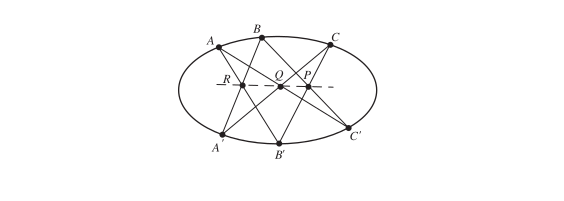
\includegraphics[width=\linewidth]{pictures/pascal.png}
  \caption{Figure from \cite{brannan}.}
  \label{fig:pascal}
\end{figure}

\begin{proof}
  We know that any non-degenerate conic can pe transformed to the standard conic. Let the conic
  be in the standard form $xy+yz+zx=0$, with $A=[1:0:0]$, $B=[0:1:0]$, and $C=[0:0:1]$. Let the
  point $A'=[a^2+a:a+1:-a]$, $B'=[b^2+b:b+1:-b]$, and $C'=[c^2+c:c+1:-c]$, for some $a,b,c\in\R$

  The line $BC'$ has the equation $x=-(c+1)z$, and the line $B'C$ has the equation $x=by$. The
  point $P$ lies on both of these lines. Hence it has the homogeneous coordinates
  $[b(c+1):c+1:-b]$. Similarly, $Q=[a(c+1):c+1:-c]$, and $R=[b(a+1):b+1:-b]$.

  To check their collinearity, evaluate the determinant:
  \[
    \begin{vmatrix}
      b(c+1) & c+1 & -b \\
      a(c+1) & c+1 & -c \\
      b(a+1) & b+1 & -b \\
    \end{vmatrix}
  \]
  Which, after some row operations, simplifies to be equal to $0$.
  Hence, the points $P$, $Q$, and $R$ are collinear.
\end{proof}

Proof adapted from \cite{brannan}.

\section{Cross-Ratio}

\begin{definition}
  Let $a$, $b$, $c$ and $d$ be four points on a projective line $D$. There exists a unique map
  from $D$ to $K\cup\{\infty\}$ that maps $a$ to $\infty$, $b$ to $0$, and $c$ to $1$. The
  image of $d$ under this projective mapping is called the \textit{cross-ratio} of the points
  $(a,b,c,d)$, and denoted $[a,b,c,d]$.
\end{definition}

\begin{prop}
  Let $a_1$, $a_2$, $a_3$, and $a_4$ be four points on the line $D$ (the first three being
  distinct) and $a'_1$, $a'_2$, $a'_3$, and $a'_4$ be four points on another line $D'$
  (satisfying the same assumption). There exists a projective transformation $f\colon D \to D'$
  such that $f(a_i)=a'_i$ iff $[a_1,a_2,a_3,a_4]=[a'_1,a'_2,a'_3,a'_4]$.
\end{prop}

\begin{proof}
  Assume $f$ is a projective mapping that sends $a_i$ to $a'_i$. Let $g$ and $g'$ be functions
  such that $[a_1,a_2,a_3,a_4]=g(a_4)$, and $[a'_1,a'_2,a'_3,a'_4]=g'(a'_4)$. $g'\circ f$ is a
  function, which maps $a_1$ to $\infty$, $a_2$ to $0$, and $a_3$ to $1$. But such function is
  unique. Hence, $g=g'\circ f$, which implies that $g(a_4)=g'(a'_4)$. That is,
  \[
    [a_1,a_2,a_3,a_4]=[a'_1,a'_2,a'_3,a'_4]
  \]
\end{proof}

\begin{remark} \textbf{Formulae for cross-ratio}\\
  Let $a$, $b$, and $c$ be four points on the affine line, the first three being distinct. Then
  \[
    [a,b,c,d]=\frac{(d-b)(c-a)}{(d-a)(c-b)}
  \]
  Also, since the points $a$ and $b$ are distinct, $c$ and $d$ can be written as
  \begin{align*}
    c=\alpha a+\beta b \\
    d=\gamma a+\delta b
  \end{align*}
  Then the cross-ratio
  \[
    [a,b,c,d]=\frac{\gamma\beta}{\alpha\delta}
  \]
\end{remark}

\begin{prop}
  If $a$, $b$, $c$, and $d$ are four distinct collinear points, then the following equalities
  hold:
  \begin{align*}
    &\left[a,b,c,d\right]+\left[a,c,b,d\right]=1 \\
    &\left[b,a,c,d\right]=\left[a,b,c,d\right]^{-1} \\
    &\left[a,b,d,c\right]=\left[a,b,c,d\right]^{-1}
  \end{align*}
\end{prop}

\begin{proof}
  Let $f$ be the function that defines the cross-ratio, such that $[a,b,c,d]=f(d)$, and let
  $f'$ be a function such that $f'(x)=1-f(x)\ \forall\,x$. The composite function $f'\circ f$ maps
  $a$ to $\infty$, $b$ to $0$, and $c$ to $1$. But the function that defines the cross-ratio
  $[a,c,b,d]$ also maps $a$ to $\infty$, $b$ to $0$, and $c$ to $1$. Since such function is
  unique,
  \begin{align*}
    [a,c,b,d] &= f'\circ f(d) \\
    \implies [a,c,b,d] &= 1-[a,b,c,d]
  \end{align*}

  Let $g$ be a function such that $g(x)=\frac{1}{f(x)}\ \forall\,x$. The composite function
  $g\circ f$ maps $a$ to $0$, $b$ to $\infty$, and $c$ to $1$. Thus it is the function that
  defines the cross-ratio $[b,a,c,d]$. That is,
  \begin{align*}
    [b,a,c,d] &= g\circ f(d) \\
    \implies [b,a,c,d] &= \frac{1}{f(d)} \\
                       &= [a,b,c,d]^{-1}
  \end{align*}

  Let $h$ be a function such that $h(x)=\frac{f(x)}{f(d)}\ \forall\,x$. The composite function
  $h\circ f$ maps $d$ to $1$, keeping the images of $a$ and $b$ unchanged. Hence, it is the
  defining function of the cross-ratio $[a,b,d,c]$. That is,
  \begin{align*}
    [a,b,d,c] &= h\circ f(c) \\
    \implies [a,b,d,c] &= \frac{f(c)}{f(d)} \\
                       &= [a,b,c,d]^{-1}
  \end{align*}
\end{proof}

\begin{remark}
  If $[a,b,c,d]=k$, the 24 cross-ratios obtained by permuting the four points take six values
  in general:
  \[
    k \hspace{8pt},\hspace{8pt} \frac{1}{k} \hspace{8pt},
    \hspace{8pt} 1-k \hspace{8pt},\hspace{8pt} 1-\frac{1}{k} \hspace{8pt},
    \hspace{8pt} \frac{1}{1-k} \hspace{8pt},\hspace{8pt} \frac{k}{k-1}
  \]
\end{remark}

\section{Group Law on Cubics}

Throughout this section, a projective cubic curve means a non-degenerate,
non-singular, non-empty projective cubic curve (i.e. its points are solutions of
a cubic polynomial in the coordinates) in a two dimensional projective
space. The following proof is adapted from \cite{silver}.

\vspace{1ex}

\noindent
Given a projective cubic curve $\mathcal{C}$ with a given point $O$ on it.
The addition law is defined as follows:

To add P and Q, take the third intersection point $P*Q$, join it to $O$ by a line, and then take the third intersection point to be $P+Q$. In other words, set $P + Q := O*(P*Q)$
In case of $P=Q$, the line passing through $P$ and $Q$ is taken to be the tangent to $\mathcal{C}$ at $P$.

\begin{figure}[H]
  \centering
  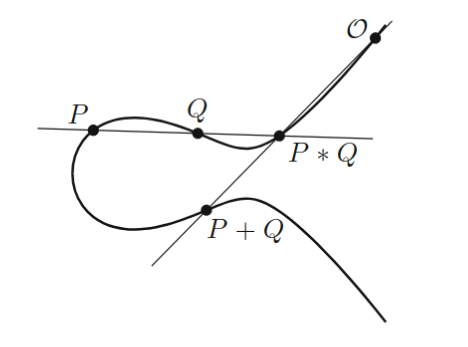
\includegraphics[width=0.5\linewidth]{pictures/Grouplaw.png}
\end{figure}

In short, we consider a point to intersect a line twice if it is tangent to the curve and thrice if the point is an inflection point. 

\noindent
Note that
\[P*Q=R \iff Q*R=P \iff R*P=Q\]
Now, we verify that the above addition rule with the set of points on $\mathcal{C}$ does indeed form a group.

\subsection*{Closure}
First, we see that the set is closed under the operation $*$.
From B\`ezout's theorem \cite[Thm.~A.1]{silver}, we can say that given two points on $\mathcal{C}$, there is a third point that intersects with the curve and line through the previous point which proves $\mathcal{C}$ is closed under $*$.
Thus, for any two points $P$ and $Q$ that lie on $\mathcal{C}$, $P+Q := O*(P*Q)$ also lies on $\mathcal{C}$.

\subsection*{Identity}
For any $P$, we have
\[P+O = O*(O*P) = P\]
which shows that $O$ is the identity element and it belongs to $\mathcal{C}$.

\subsection*{Inverse}
Let $S:=O*O$. For any point $Q$, consider $Q+(Q*S)$ as
\[Q+(Q*S) = O*(Q*(Q*S)) = O*S = O\]
$(Q*S)$ exists if $S$ exists which is true due to B\`ezout's theorem \cite[Thm.~A.1]{silver}.
If $O$ is an inflection point, then $S = O$.
Thus, the inverse of $Q$ is $(Q*S)$ which lies on $\mathcal{C}$.

\subsection*{Associativity}

We define the following lines:
\begin{align*}
  l_1 &\colon \text{Passes through }Q,\ R,\ Q*R   & m_1 &\colon \text{Passes through }P,\ Q,\ P*Q \\
  l_2 &\colon \text{Passes through }O,\ P*Q,\ P+Q & m_2 &\colon \text{Passes through }O,\ Q*R,\ Q+R \\
  l_3 &\colon \text{Passes through }P,\ Q+R       & m_3 &\colon \text{Passes through }R,\ P+R
\end{align*}
Because the curve is in the projective plane, the point of intersection of lines $l_3$ and $m_3$ always exists; let that point be $T$.
Now, we consider the cubic curve obtained by multiplying the equations of $l_1$,$l_2$ and $l_3$ as $L$.
Similarily, we consider the curve obtained from $m_1$, $m_2$, $m_3$ as $M$.
They will  meet at 9 points due to B\`ezout's theorem \cite[Thm.~A.1]{silver} which are:
\[O,\ P,\ Q,\ R,\ P*Q,\ Q*R,\ P+Q,\ Q+R,\ T\]
\begin{figure}[H]
  \centering
  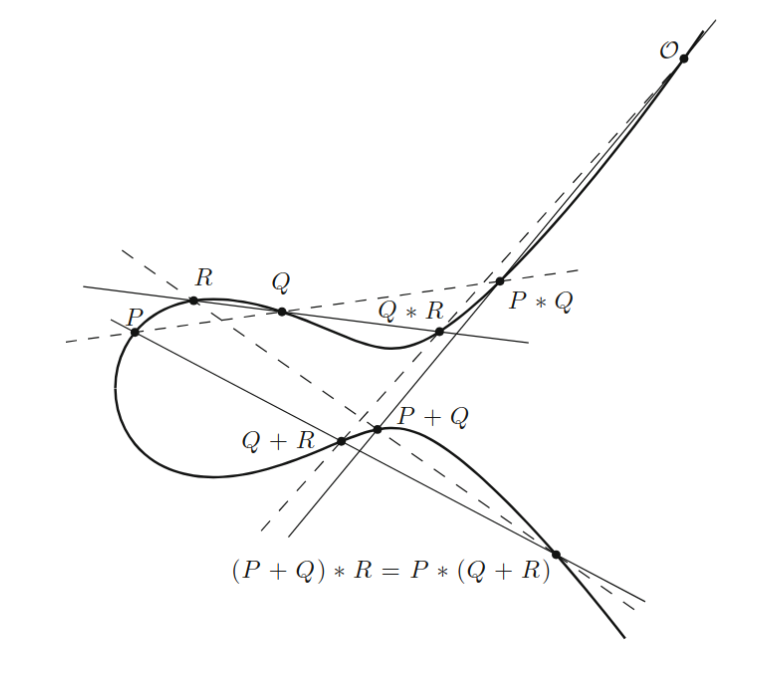
\includegraphics[width=0.7\linewidth]{pictures/Associativity.png}
  \caption{Solid lines represents $L$ while dotted lines represents $M$}
\end{figure}
But we see that the cubic curve $\mathcal{C}$ passes through all of these points except $T$.
From the Cayley-Bacharach theorem \cite[Thm.~A.3]{silver}, if two cubic curves $L$ and $M$ intersect at 9 points and another cubic curve $\mathcal{C}$ passes through 8 of those points then it passes through the ninth point as well.
Hence, $T$ lies on $\mathcal{C}$.

\vspace{1ex}

\noindent
Consider the points of intersection between $\mathcal{C}$ and $l_3$.
$P$ and $Q+R$ lie on both of them, thus the third point of intersection will be $P*(Q+R)$, which happens to be $T$.

\vspace{1ex}

Similarly, looking at the points of intersection between $\mathcal{C}$ and $m_3$, we see that the point $T$ also happens to be $(P+Q)*R$.

\vspace{1ex}

\noindent
Because they are the same point, we have that:
\[(P+Q)*R = P*(Q+R)\]
From which we can conclude that
\[(P+Q)+R = P+(Q+R)\]
Thus, the points of $\mathcal{C}$ form a group under the operation $+$.
